%%%%%%%%%%%%%%%%%%%%%%%%%%%%%%%%%%%%%%%%%
% Arsclassica Article
% LaTeX Template
% Version 1.1 (1/8/17)
%
% This template has been downloaded from:
% http://www.LaTeXTemplates.com
%
% Original author:
% Lorenzo Pantieri (http://www.lorenzopantieri.net) with extensive modifications by:
% Vel (vel@latextemplates.com)
%
% License:
% CC BY-NC-SA 3.0 (http://creativecommons.org/licenses/by-nc-sa/3.0/)
%
%%%%%%%%%%%%%%%%%%%%%%%%%%%%%%%%%%%%%%%%%

%----------------------------------------------------------------------------------------
%	PACKAGES AND OTHER DOCUMENT CONFIGURATIONS
%----------------------------------------------------------------------------------------

\documentclass[
12pt, % Main document font size
a4paper, % Paper type, use 'letterpaper' for US Letter paper
oneside, % One page layout (no page indentation)
%twoside, % Two page layout (page indentation for binding and different headers)
headinclude,footinclude, % Extra spacing for the header and footer
BCOR5mm, % Binding correction
]{scrartcl}
\usepackage[english]{babel}
\usepackage{url}
\usepackage{graphicx}
\usepackage{subcaption}
%%%%%%%%%%%%%%%%%%%%%%%%%%%%%%%%%%%%%%%%%
% Arsclassica Article
% Structure Specification File
%
% This file has been downloaded from:
% http://www.LaTeXTemplates.com
%
% Original author:
% Lorenzo Pantieri (http://www.lorenzopantieri.net) with extensive modifications by:
% Vel (vel@latextemplates.com)
%
% License:
% CC BY-NC-SA 3.0 (http://creativecommons.org/licenses/by-nc-sa/3.0/)
%
%%%%%%%%%%%%%%%%%%%%%%%%%%%%%%%%%%%%%%%%%

%----------------------------------------------------------------------------------------
%	REQUIRED PACKAGES
%----------------------------------------------------------------------------------------

\usepackage[
nochapters, % Turn off chapters since this is an article        
beramono, % Use the Bera Mono font for monospaced text (\texttt)
eulermath,% Use the Euler font for mathematics
pdfspacing, % Makes use of pdftex’ letter spacing capabilities via the microtype package
dottedtoc % Dotted lines leading to the page numbers in the table of contents
]{classicthesis} % The layout is based on the Classic Thesis style

\usepackage{arsclassica} % Modifies the Classic Thesis package

\usepackage[T1]{fontenc} % Use 8-bit encoding that has 256 glyphs

\usepackage[utf8]{inputenc} % Required for including letters with accents

\usepackage{graphicx} % Required for including images
\graphicspath{{Figures/}} % Set the default folder for images

\usepackage{enumitem} % Required for manipulating the whitespace between and within lists

\usepackage{lipsum} % Used for inserting dummy 'Lorem ipsum' text into the template

%\usepackage{subfig} % Required for creating figures with multiple parts (subfigures)

\usepackage{amsmath,amssymb,amsthm} % For including math equations, theorems, symbols, etc

\usepackage{varioref} % More descriptive referencing

%----------------------------------------------------------------------------------------
%	THEOREM STYLES
%---------------------------------------------------------------------------------------

\theoremstyle{definition} % Define theorem styles here based on the definition style (used for definitions and examples)
\newtheorem{definition}{Definition}

\theoremstyle{plain} % Define theorem styles here based on the plain style (used for theorems, lemmas, propositions)
\newtheorem{theorem}{Theorem}

\theoremstyle{remark} % Define theorem styles here based on the remark style (used for remarks and notes)

%----------------------------------------------------------------------------------------
%	HYPERLINKS
%---------------------------------------------------------------------------------------

\hypersetup{
%draft, % Uncomment to remove all links (useful for printing in black and white)
colorlinks=true, breaklinks=true, bookmarks=true,bookmarksnumbered,
urlcolor=webbrown, linkcolor=RoyalBlue, citecolor=webgreen, % Link colors
pdftitle={}, % PDF title
pdfauthor={\textcopyright}, % PDF Author
pdfsubject={}, % PDF Subject
pdfkeywords={}, % PDF Keywords
pdfcreator={pdfLaTeX}, % PDF Creator
pdfproducer={LaTeX with hyperref and ClassicThesis} % PDF producer
} % Include the structure.tex file which specified the document structure and layout

\hyphenation{Fortran hy-phen-ation} % Specify custom hyphenation points in words with dashes where you would like hyphenation to occur, or alternatively, don't put any dashes in a word to stop hyphenation altogether

%----------------------------------------------------------------------------------------
%	TITLE AND AUTHOR(S)
%----------------------------------------------------------------------------------------

\title{\normalfont{disCOVIDer19}} % The article title

\subtitle{A path-guide inside the COVID-19 pandemia } % Uncomment to display a subtitle

\author{Fabio Caironi, Marzio De Corato, \\
Andrea Ierardi, Federico Matteucci,\\
 Gregorio Saporito} % The article author(s) - author affiliations need to be specified in the AUTHOR AFFILIATIONS block

\date{} % An optional date to appear under the author(s)

%----------------------------------------------------------------------------------------

\begin{document}

%----------------------------------------------------------------------------------------
%	HEADERS
%----------------------------------------------------------------------------------------

\renewcommand{\sectionmark}[1]{\markright{\spacedlowsmallcaps{#1}}} % The header for all pages (oneside) or for even pages (twoside)
%\renewcommand{\subsectionmark}[1]{\markright{\thesubsection~#1}} % Uncomment when using the twoside option - this modifies the header on odd pages
\lehead{\mbox{\llap{\small\thepage\kern1em\color{halfgray} \vline}\color{halfgray}\hspace{0.5em}\rightmark\hfil}} % The header style

\pagestyle{scrheadings} % Enable the headers specified in this block

%----------------------------------------------------------------------------------------
%	TABLE OF CONTENTS & LISTS OF FIGURES AND TABLES
%----------------------------------------------------------------------------------------

\maketitle % Print the title/author/date block

\setcounter{tocdepth}{2} % Set the depth of the table of contents to show sections and subsections only

\tableofcontents % Print the table of contents

\listoffigures % Print the list of figures

\listoftables % Print the list of tables

%----------------------------------------------------------------------------------------
%	ABSTRACT
%----------------------------------------------------------------------------------------

\section*{Abstract} % This section will not appear in the table of contents due to the star (\section*)



%----------------------------------------------------------------------------------------
%	AUTHOR AFFILIATIONS
%----------------------------------------------------------------------------------------

%\let\thefootnote\relax\footnotetext{* \textit{Department of Biology, University of Examples, London, United Kingdom}}

%\let\thefootnote\relax\footnotetext{\textsuperscript{1} \textit{Department of Chemistry, University of Examples, London, United Kingdom}}

%----------------------------------------------------------------------------------------

\newpage % Start the article content on the second page, remove this if you have a longer abstract that goes onto the second page

%----------------------------------------------------------------------------------------
%	INTRODUCTION
%----------------------------------------------------------------------------------------

\section{Introduction} \label{introduction}

\paragraph{Background} \label{Background}
In December 2019 different cases of pneumonia were reported in Wuhan (China) \cite{huang2020clinical}. Their origin was later ascribed to a new virus classified as \textit{Severe acute respiratory syndrome coronavirus 2} (SARS-CoV-2) whose TEM and SEM pictures are reported in the Fig. \ref{coronavirus_picture} The origin of this virus is still subject of scientific debate between the scientific community, however one of the most common opinion is that this virus comes from bats, in particular the genus Rhinolophus \cite{zhou2020pneumonia}. The most compelling feature of this virus is that is its ability to spread also via coughing and sneezing \cite{ghinai2020first}, and also by touching infected surfaces \cite{chang2020protecting}. Differently with respect to the SARS-CoV the virus seems to have a lower mortality rate \cite{sorensen2006severe,weiss2020clinical}.



\begin{figure}[ht]
\begin{subfigure}{.5\textwidth}
  \centering
  % include first image
  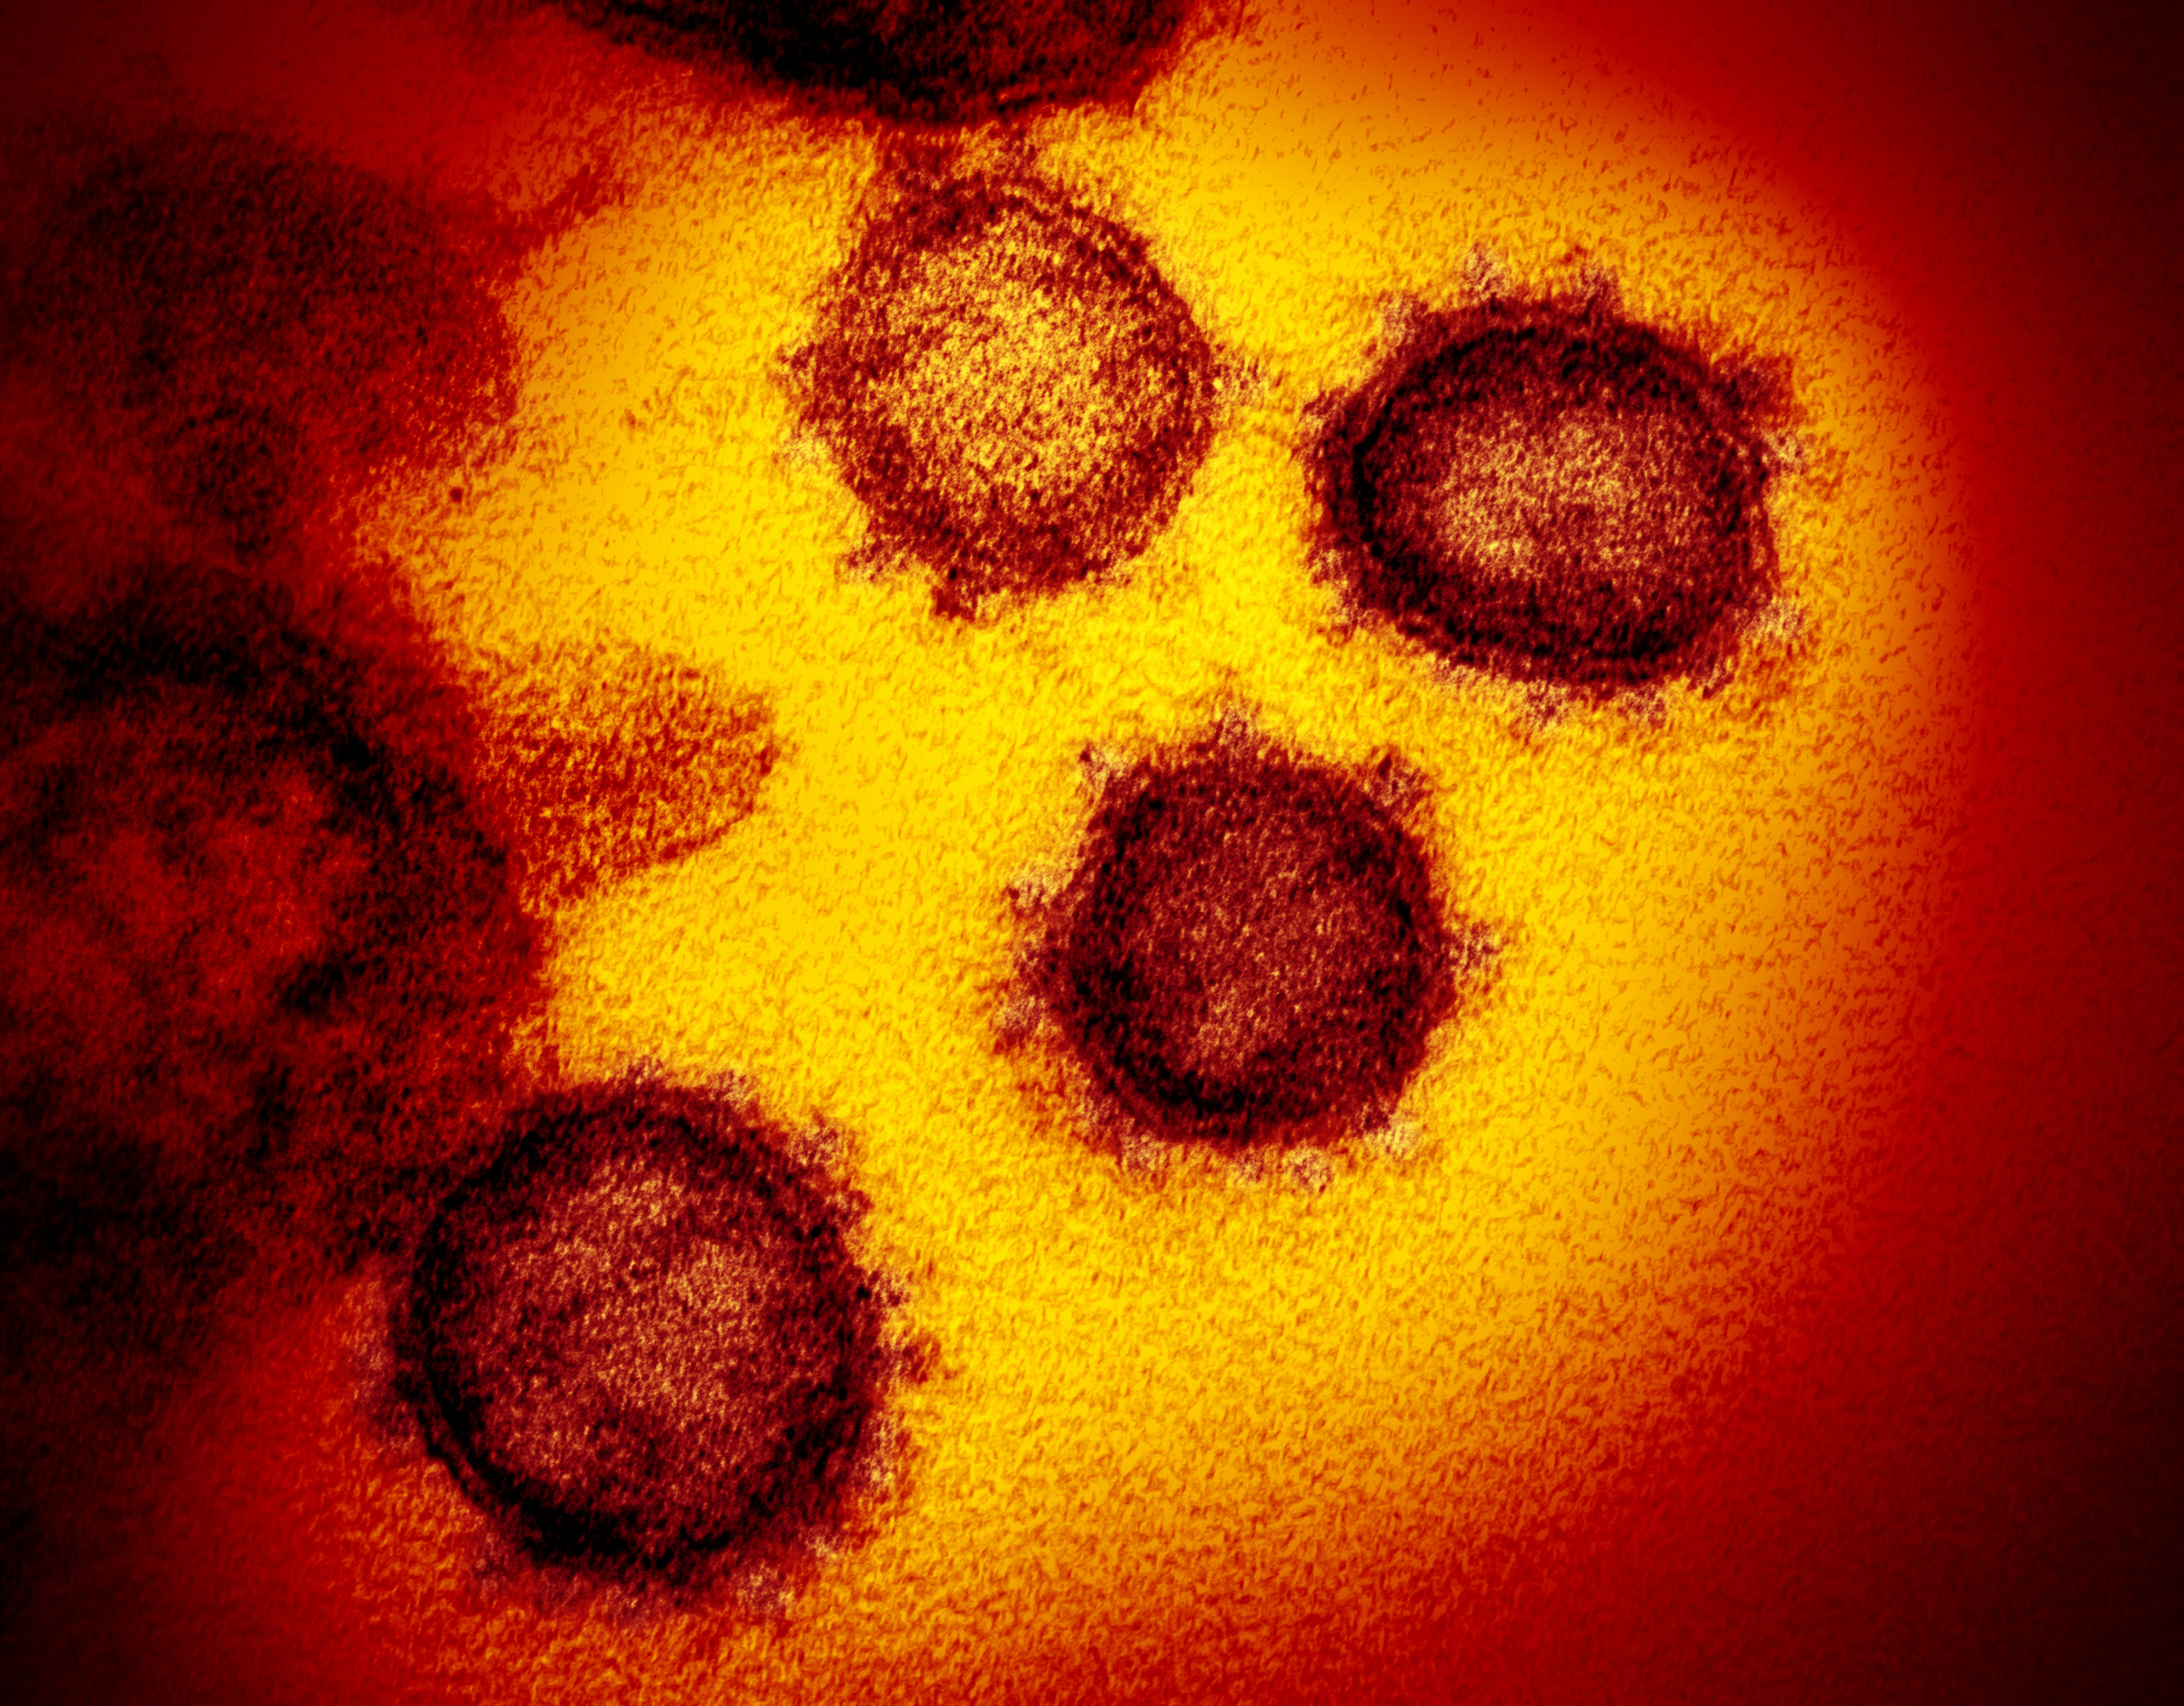
\includegraphics[width=.7\linewidth]{Figures/Coronavirus1.jpg}
  \caption{Transmission electron microscope (TEM) image of SARS-CoV-2—also known as 2019-nCoV, emerging from the surface of cells cultured}
  \label{fig:sub-first}
\end{subfigure}
\begin{subfigure}{.5\textwidth}
  \centering
  % include second image
  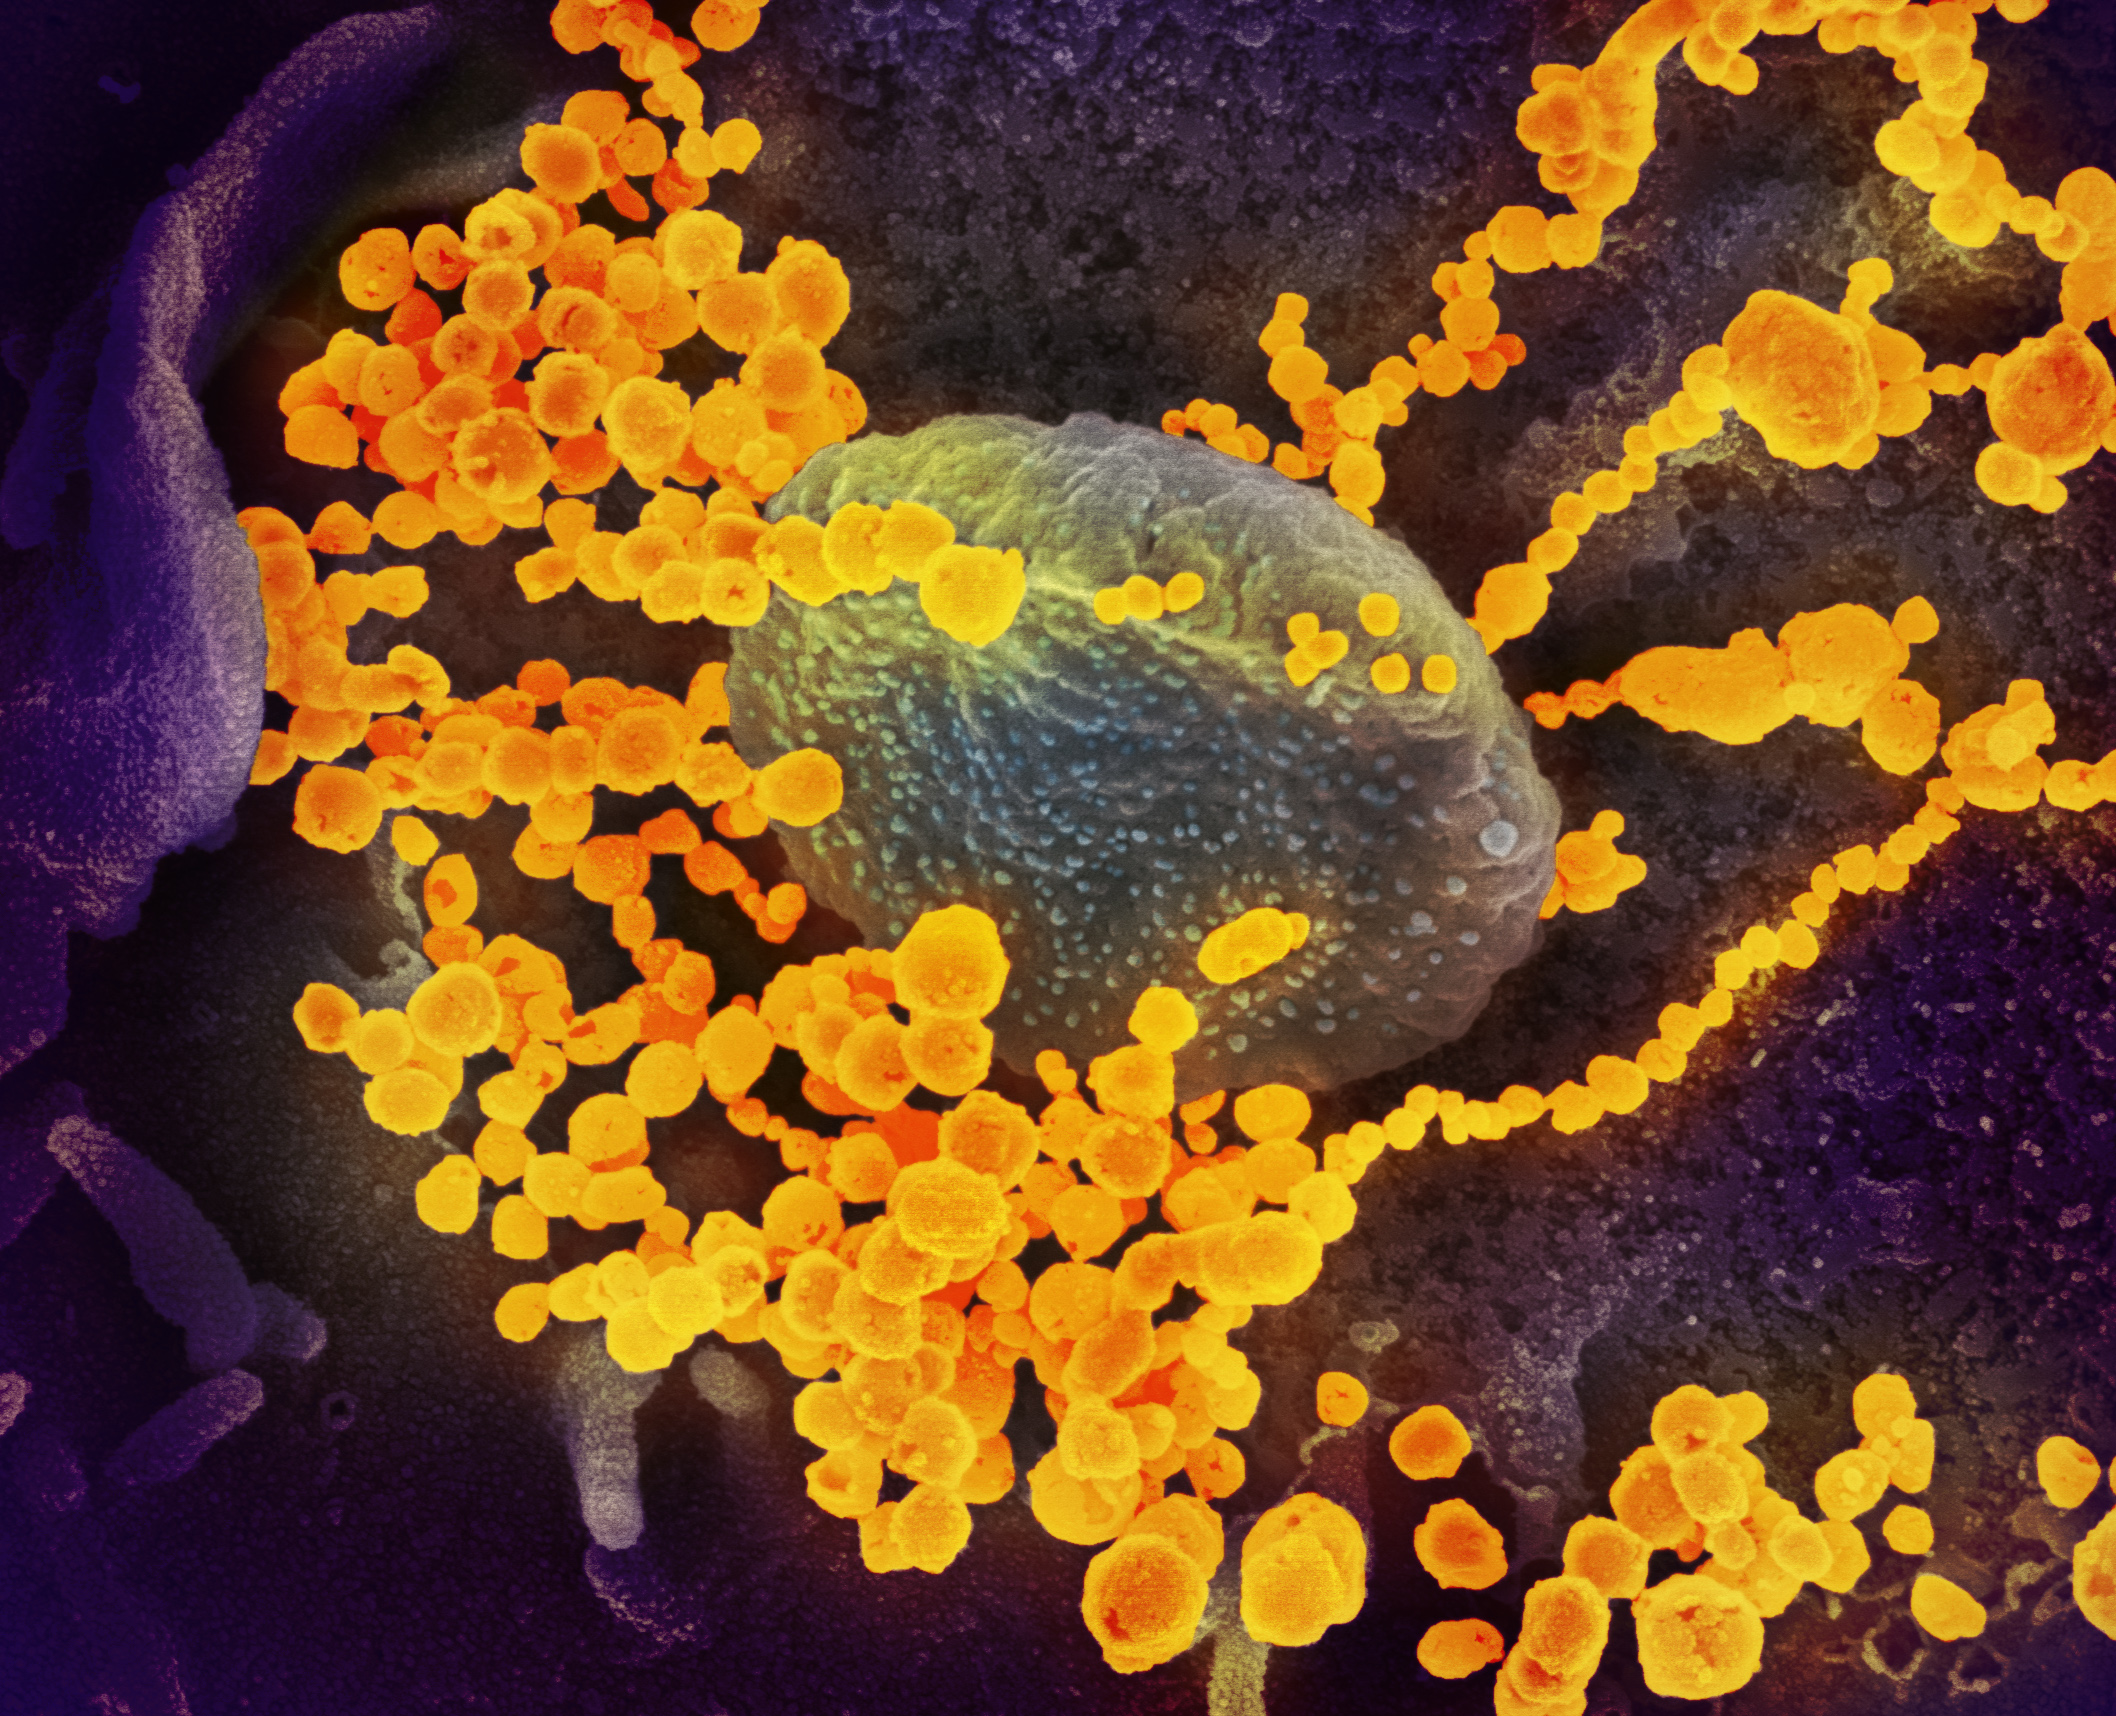
\includegraphics[width=.7\linewidth]{Figures/Coronavirus2.jpg} 
  \caption{Scanning electron microscope of the SARS-CoV-2 emerging from the surface of cells cultured}
  \label{fig:sub-second}
\end{subfigure}
\begin{subfigure}{.5\textwidth}
  \centering
  % include second image
  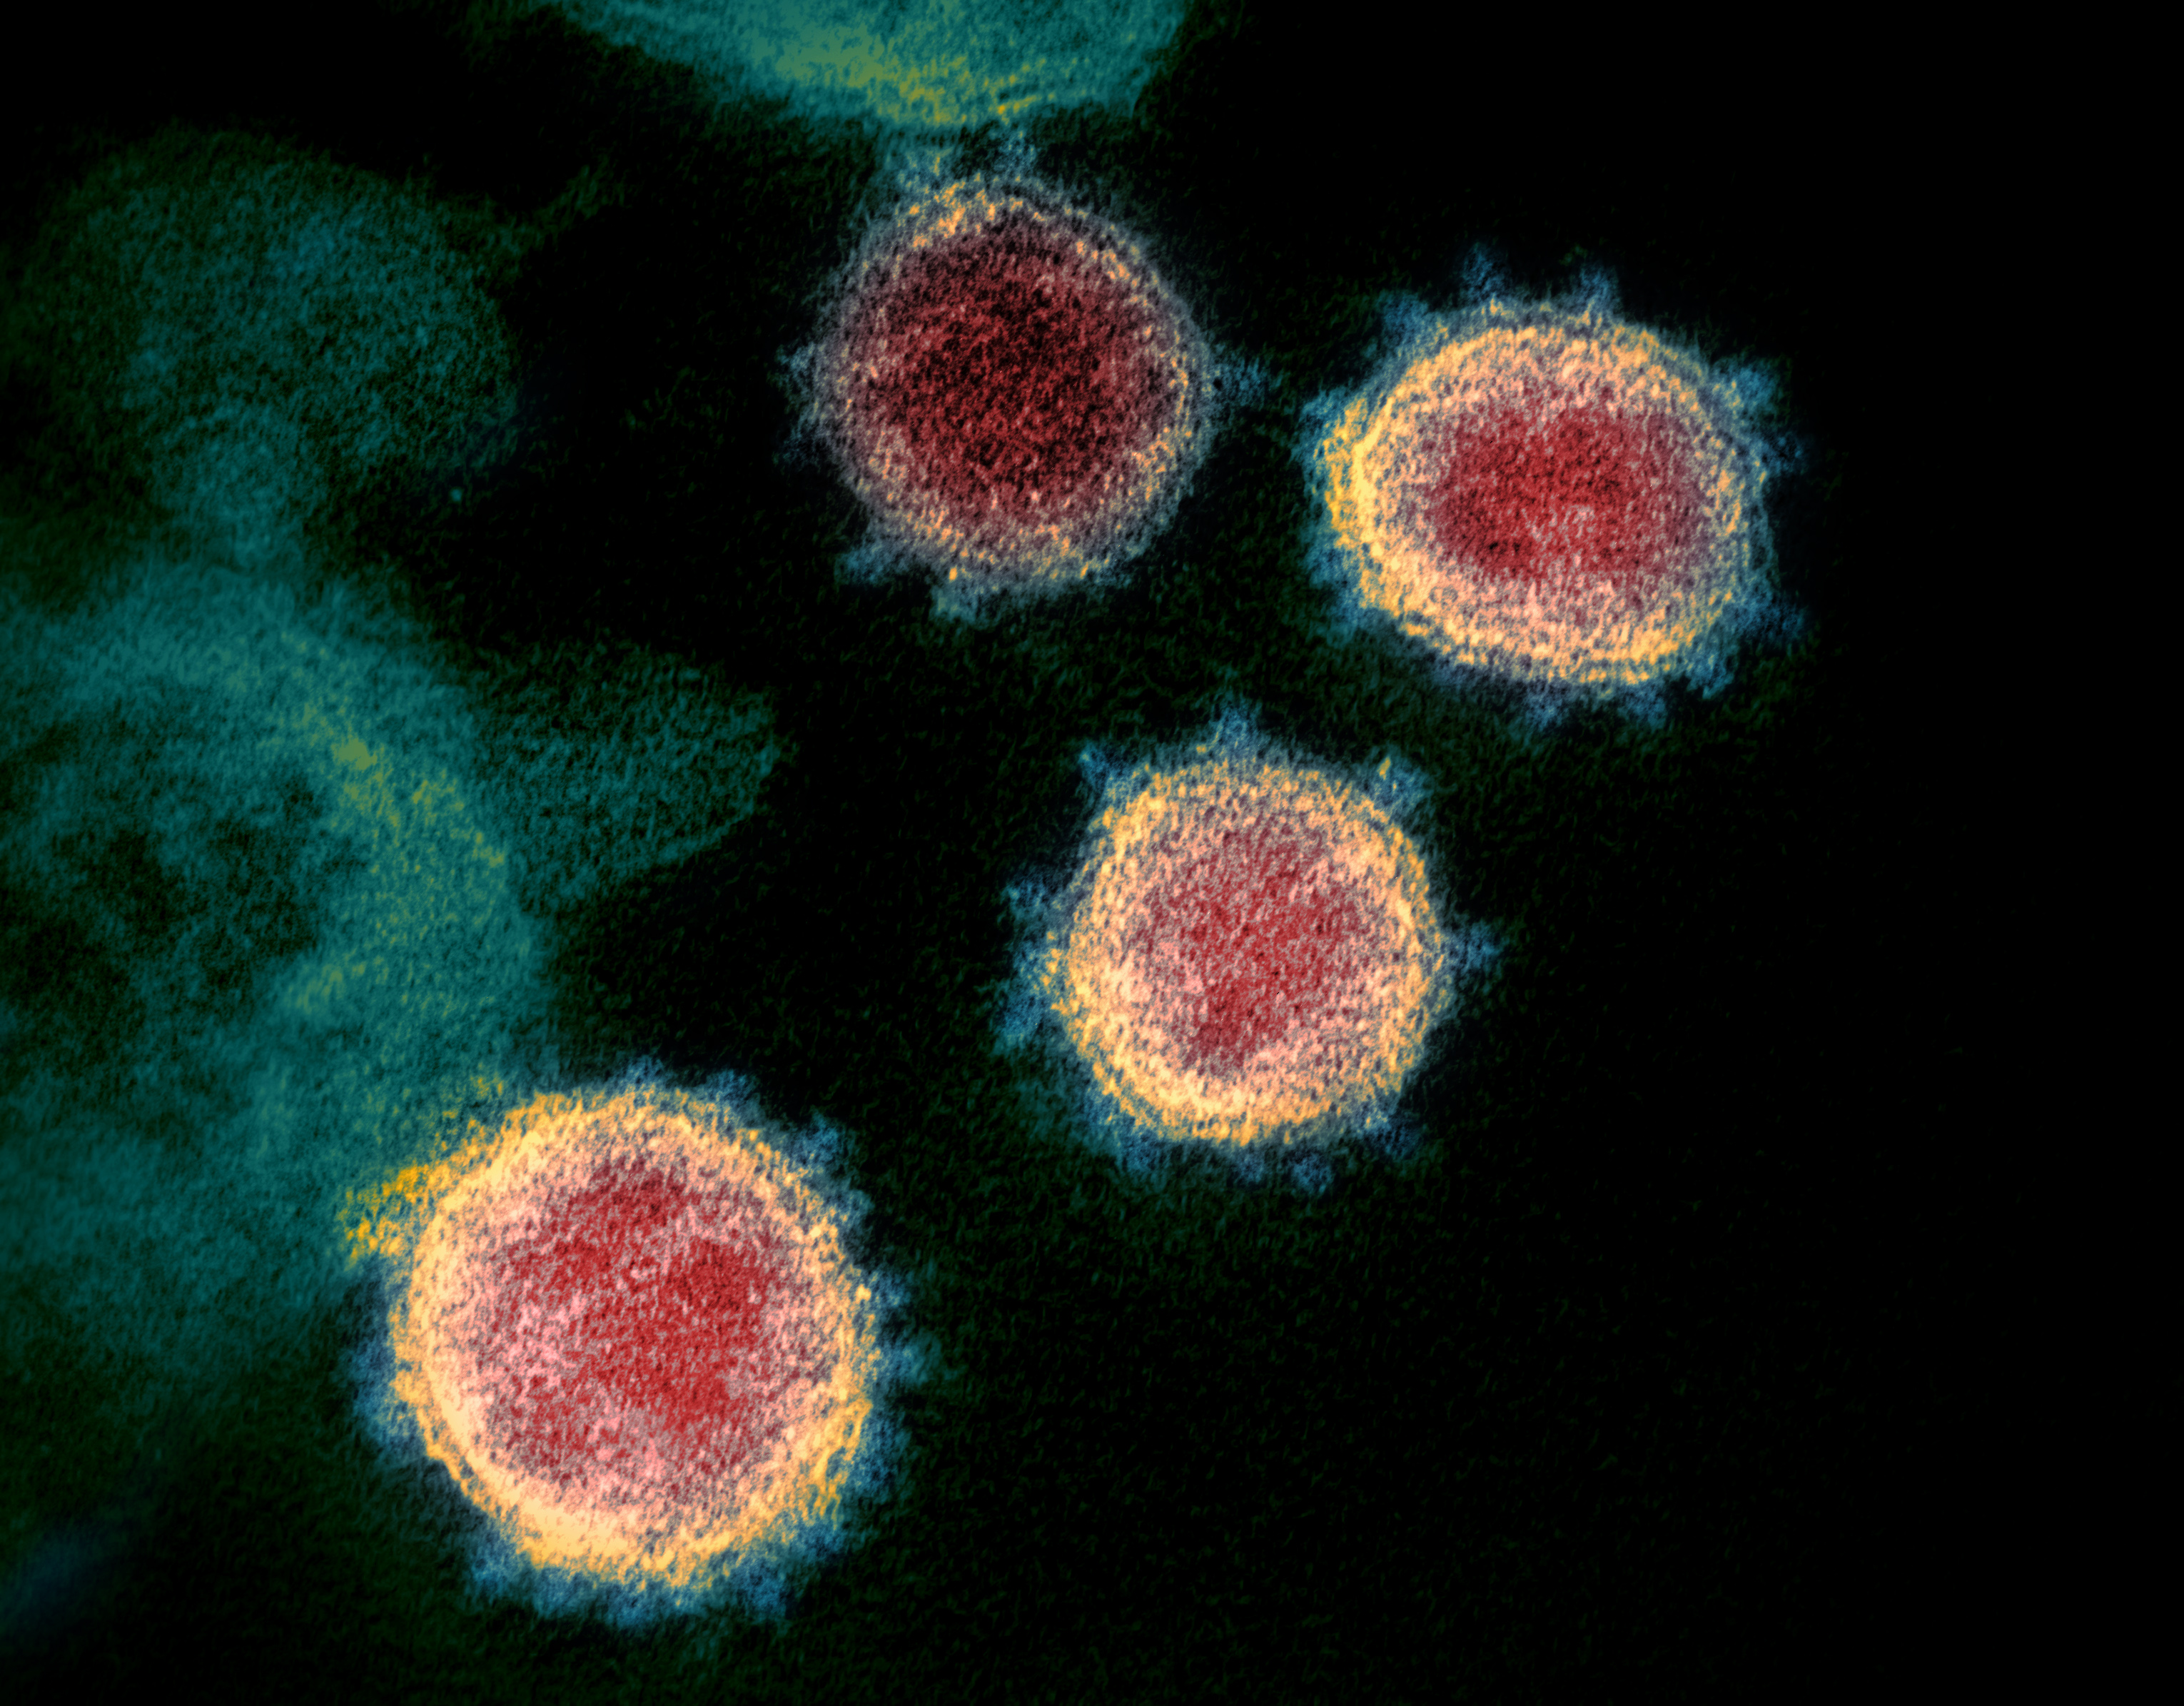
\includegraphics[width=.7\linewidth]{Figures/Coronavirus3.jpg} 
  \caption{TEM image of SARS-CoV-2. Not the spikes that gives the name coronavirus to the virus }
  \label{fig:sub-second}
\end{subfigure}
\begin{subfigure}{.5\textwidth}
  \centering
  % include second image
  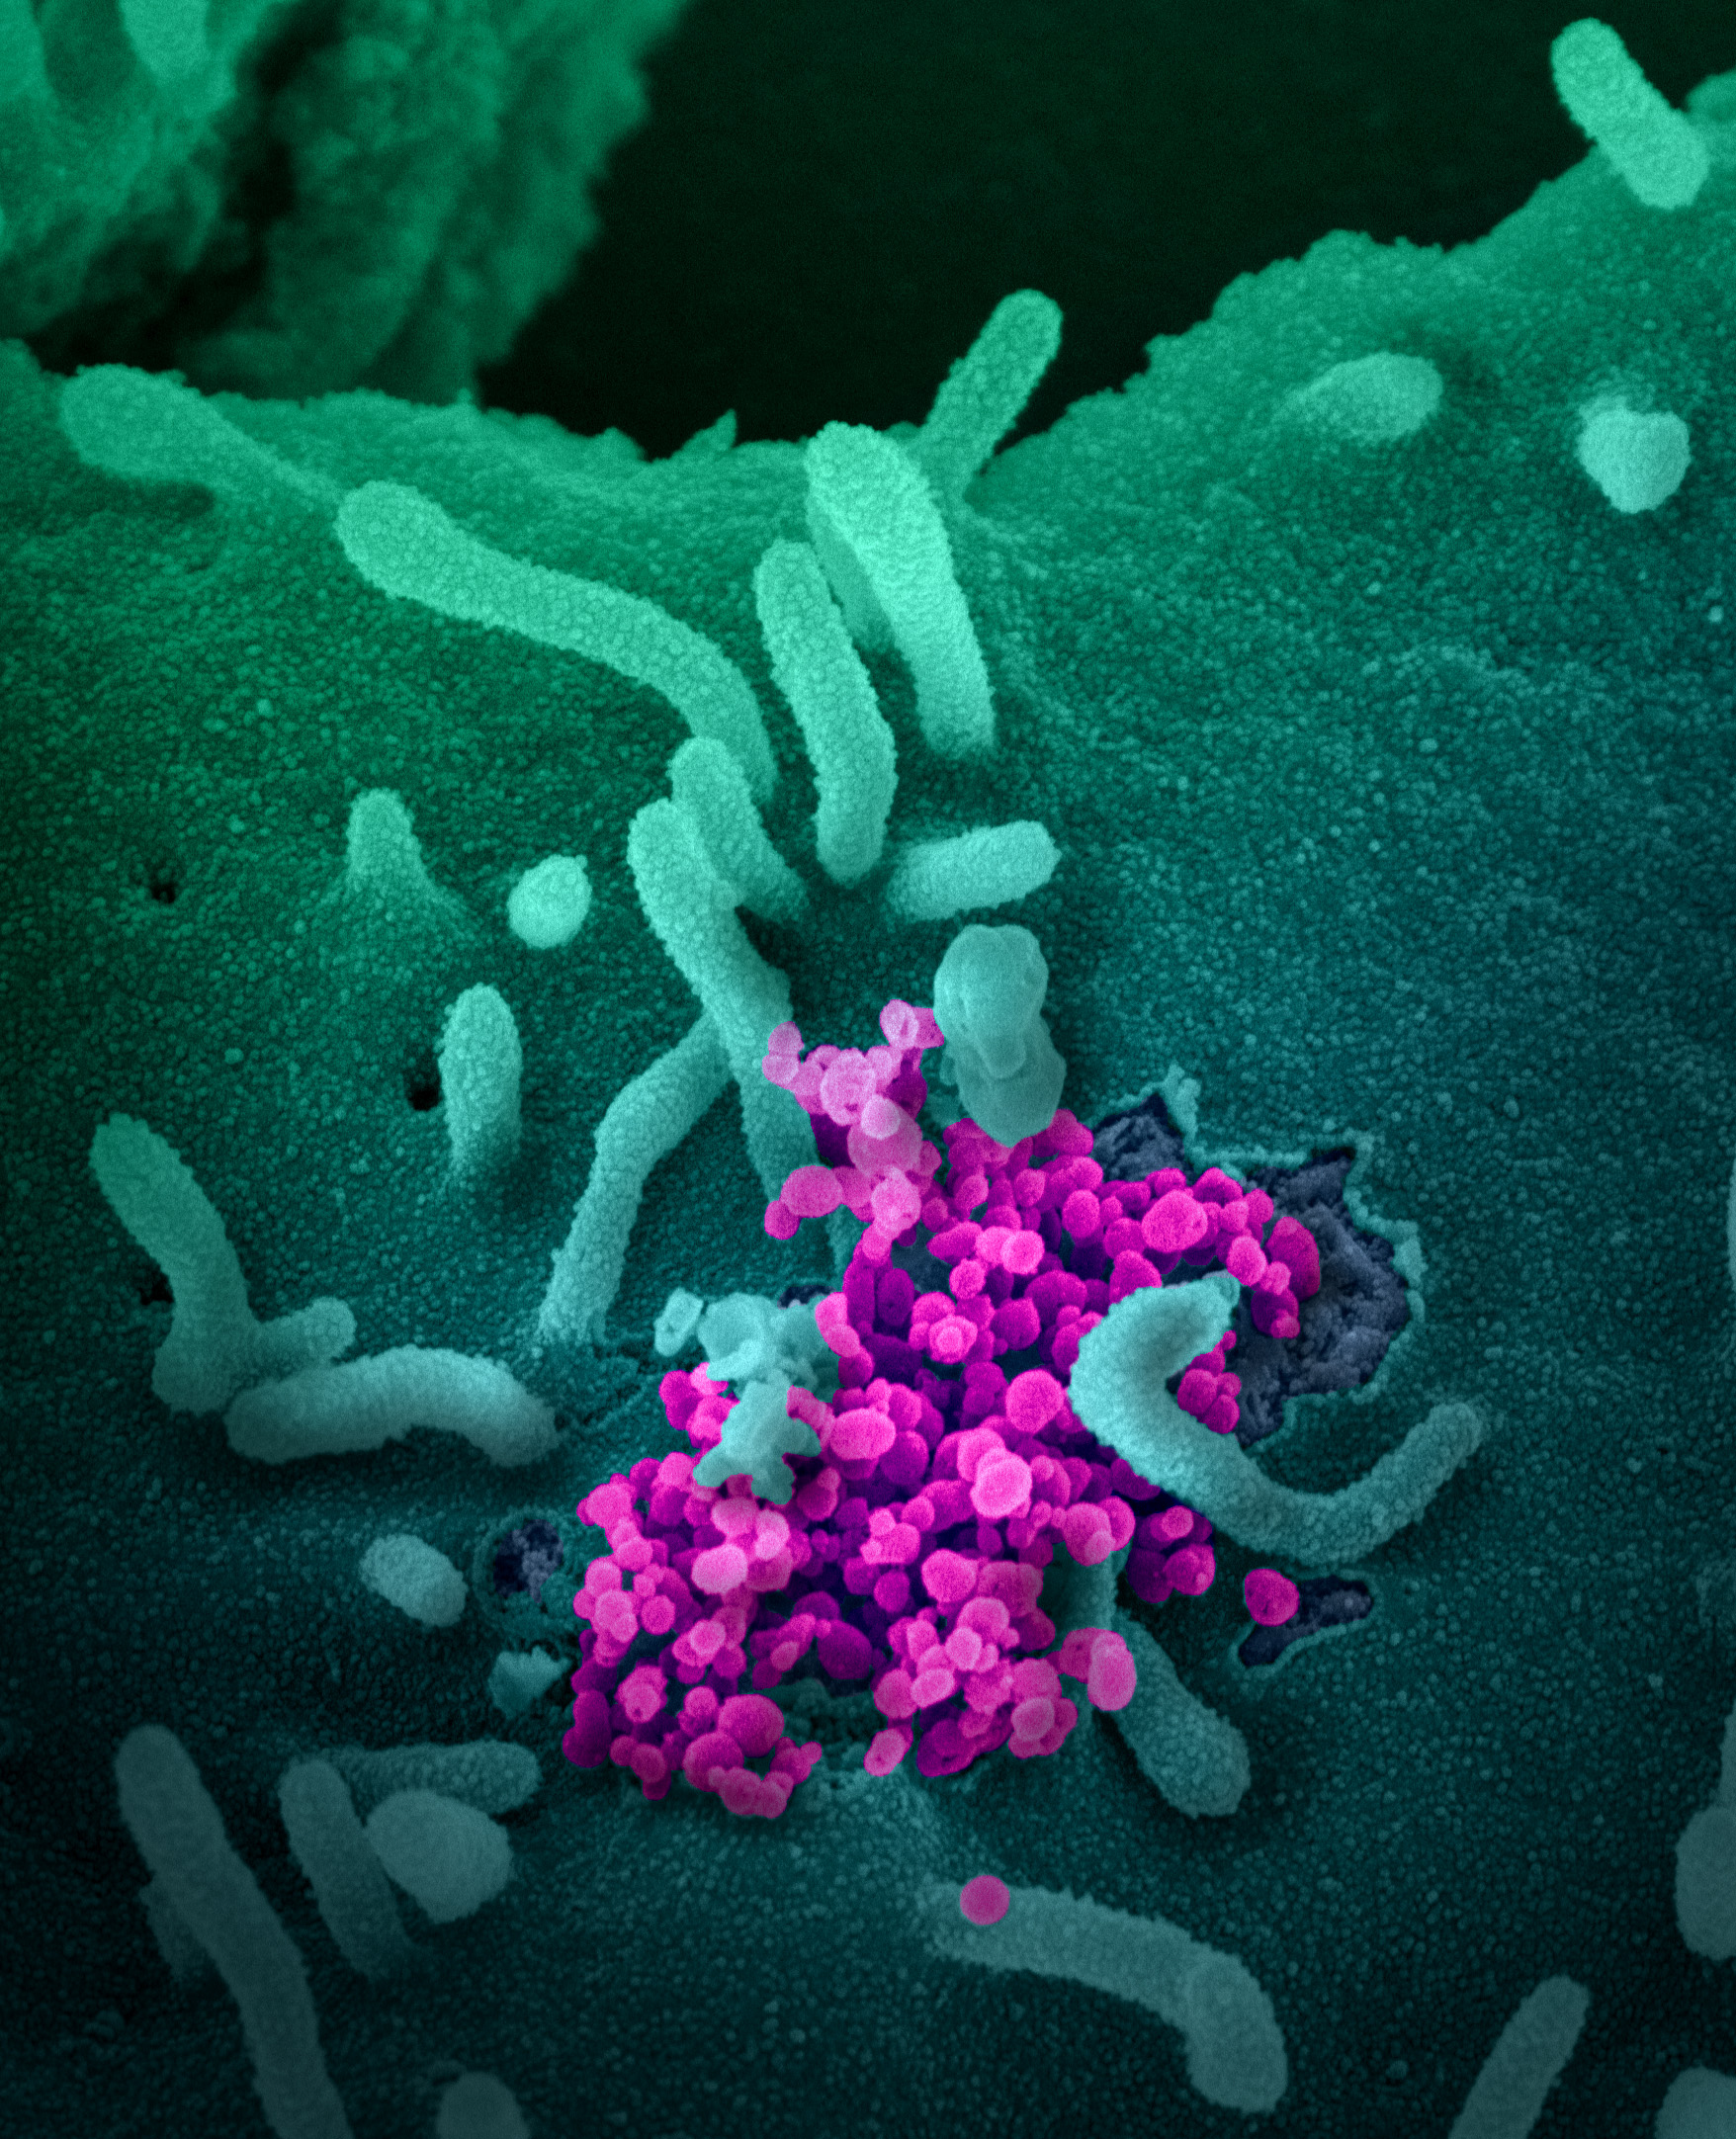
\includegraphics[width=.7\linewidth]{Figures/Coronavirus4.jpg} 
  \caption{SEM image of the virus}
  \label{fig:sub-second}
\end{subfigure}
\caption{Different pictures of the virus as reported by the NIAID’s Rocky Mountain Laboratories (RML) in Hamilton, Montana \cite{coronavirus+pictures}  }
\label{coronavirus_picture}
\end{figure}


In January the Chinese government imposed the quarantine for the city of Wuhan (almost 11M people); the quarantine was later expanded to the full province of Hubei (60M people) and then to the neighbour provinces Huanggang, Ezhou and Xianning. 
The virus then spread in Canada, Germany, Thailand and Japan and then in other different countries included Italy \cite{timeline+web}. In Italy the first cases, two Chinese tourist from Hubei, were reported in Rome \cite{corr+roma}; then  other cases were reported in Codogno (Lodi,Lombardy). Later the virus spread almost in all regions of Italy with a higher density in Lombardy, Veneto, Emilia-Romagna, Piemonte and Marche. Starting from 22 of February, the Italian government started to impose the quarantine (red-zone) for 11 different municipalities, in particular Codogno, Casalpusterlengo, Lodi (included the neighbour municipalities) and Vo' . Starting from this date different restrictive measures were imposted starting from the regions with the highest number of cases: public entrainment were almost suspended as well as schools and universities. Workers (in public and private sectors) were allowed, when possibile, to work at home (smart-working). Such measures culminated with a decree approved by the Italian government that divided Italy in three areas: the red zones in which the municipalities with highest number of cases in which all the population was subjected to quarantine, the yellow one (Lombardia, Veneto, Emilia Romagna) in which schools, universities and public events ,sports  as well cinemas were suspended and the rest of Italy in which no restrictive measures were adopted \cite{rep+dec1}; however 3 days later all schools and universities were suspended \cite{guard+01}. The restrictive measures were also extend up to all Italy with a further decree \cite{11marzo}. 

\paragraph{Motivation} \label{Motivation}
In order to have a better understanding about the spread and the effects on the population of the COVID19 disease, we propose a ShinyApp, called disCOVIDer19 , that gathers  the data , mostly provided by the Protezione Civile \cite{protezionecivile+git}, about the number of infections(current as well cumulative), hospitalized people as well in intensive care, deaths and recovered for Italy, its regions and provinces; more details will be discussed in sections \ref{Data Origin} and \ref{Panels}. Furthermore we fitted the cumulative cases for Italy and all its regions and provinces with a logistic curve, in order to get a bird-of-eye view on the trend followed as well on the effectiveness of the restrictive measures imposed by the Italian government. The theoretical foundations of this fit ,as well how to manage and use it, will be discussed in the section \ref{Theoretical Background}. Beside the logistic curve, we also considered a statistical approach, largely diffused among economists, that considers the number of cases in each day as a time series: on this basis we were able to make use of a particular tool, which will be briefly introduced in the section \ref{Theoretical Background}, that allowed us to  make a further forecast  about future cases.  This latter becomes useful in case of large deviations from logistic distribution. 
 
%----------------------------------------------------------------------------------------
%	METHODS
%----------------------------------------------------------------------------------------

\section{Theoretical Background} \label{Theoretical Background}
Different models were proposed in the literature for modelling the spread of a disease \cite{keeling2011modeling}, here we are going to consider a relative simple model taken from the growth dynamics of populations.

\paragraph{Population growth dynamics}
The dynamics of population was founded by Thomas Malthus in 1817 \cite{malthus1817essay} with his well known equation: 

\begin{equation}
x_{n+1}=x_{n}(1+r)
\end{equation}

Where $x_{n}$ stands for the population at time and $r$ the growth rate. Thus the following discrete progression will be obtained: 

\begin{equation}
P_{n+1}=P_{0}(1+r)^{n+1}
\end{equation}

in which $P_{0}$ stands for the initial population. This discrete model can be reshaped in to a continuous one in the following way: 

\begin{equation}
\dot{P}(t)=rP(t)
\end{equation}

this is a relative simple differential equation with separable variable. Its integration gives:

\begin{equation}
P(t)=P_{0}(t)
\end{equation}

Malthus, of course, did not believed that the population could grow ad infinitum with an exponential growth, but since he estimated that the resources growth follows a linear path, he argued that, at the intersection of the two curves, a consistent part of the population will not have access to the resources. Thus  he expected that the exponential growth realizes only in the first part of the growth. Basing on these arguments, a Belgian mathematician Pierre-François Verhulst in 1838, proposed a model \cite{verhulst1838notice} in which the key point is the maximum number of people that the resources allows to live, usually called the carrying capacity here indicated as $K$ ($P$ and $r$ have the same meaning of the previous model):

\begin{equation}
\dot{P}=rP\left(1-\dfrac{P}{K} \right)
\end{equation}

that have the following analytic solution 

\begin{equation}
P=\dfrac{KP_{0}e^{rt}}{K+P_{0}(e^{rt}-1)}
\end{equation}

%------------------------------------------------

\section{Data Origin} \label{Data Origin}



%------------------------------------------------

\section{Panels} \label{Panels}

\subsection{Home}

\subsection{Data Inspection}

\subsection{Data Analysis}

\section{Conclusions}

\section{Packages used}


%------------------------------------------------



%----------------------------------------------------------------------------------------
%	BIBLIOGRAPHY
%----------------------------------------------------------------------------------------

\renewcommand{\refname}{\spacedlowsmallcaps{References}} % For modifying the bibliography heading

\bibliographystyle{unsrt}

\bibliography{sample.bib} % The file containing the bibliography

%----------------------------------------------------------------------------------------

\end{document}
